\section{Assignment 8}

\subsection{Implement in Simulink the Adaptive Control law for the a 1-DoF link under gravity.}

\begin{figure}[H]
\centering
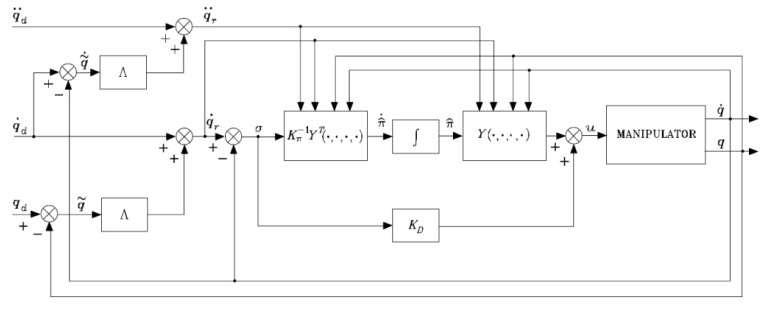
\includegraphics[keepaspectratio,width=0.6\textwidth]{adaptive_arch}
\caption{Adaptive control architecture}
\end{figure}

The adaptive control law tackles the problem of model uncertainty by implementing an on-line estimator of the robot's dynamic parameters. 

The plant is modelled with three dynamic parameters (inertia, friction and gravity term):

\begin{equation*}
I\ddot q + F\dot q + G\sin q = \tau\implies \tau = \begin{bmatrix}
\ddot q & \dot q & \sin q
\end{bmatrix}\begin{bmatrix}
I\\ F\\ G
\end{bmatrix}=Y(q,\dot q,\ddot q)\Theta
\end{equation*}

The estimation of the dynamic parameters is as follows:

\begin{equation*}
\hat\Theta=\begin{bmatrix}
\hat I\\\hat F\\\hat G
\end{bmatrix}=\begin{bmatrix}
\gamma_1 & 0 & 0\\ 0 & \gamma_2 & 0\\ 0 & 0 & \gamma_3
\end{bmatrix}\begin{bmatrix}
\ddot q\\\dot q\\\sin q
\end{bmatrix}(\dot q_r-\dot q)
\end{equation*}

where the reference velocity is computed as:

\begin{equation*}
\dot q_r = \dot q_d+\lambda (q_d-q) = \dot q_d+\frac{K_P}{K_D} (q_d-q)
\end{equation*}

The architecture is implemented in SIMULINK as follows:

\begin{figure}[H]
\centering
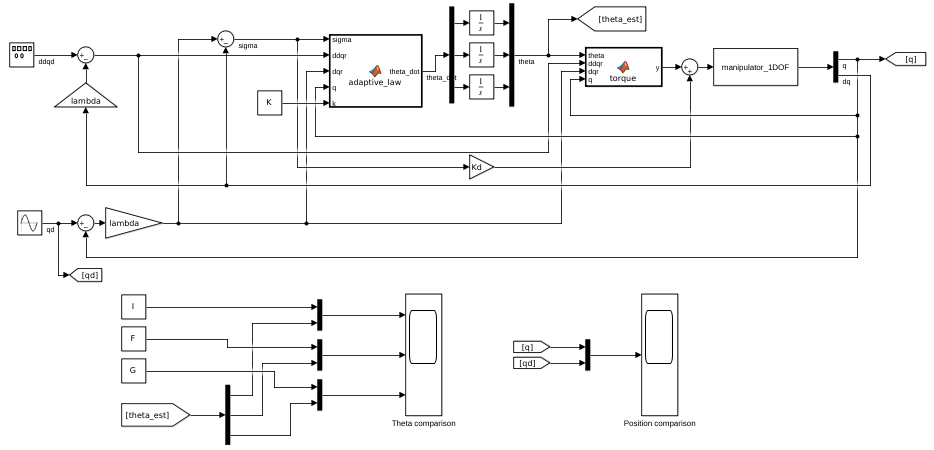
\includegraphics[keepaspectratio,width=0.6\textwidth]{adaptive_sim}
\caption{Adaptive control SIMULINK model}
\end{figure}

The model is tested with a sinusoidal reference trajectory $q_d=A\sin(\omega t)$ and a periodic square wave acceleration reference $\ddot q_d = square(\pm A)$, with $A=1$ and $\omega = 2\pi$.

\newpage

\begin{figure}[H]
\centering
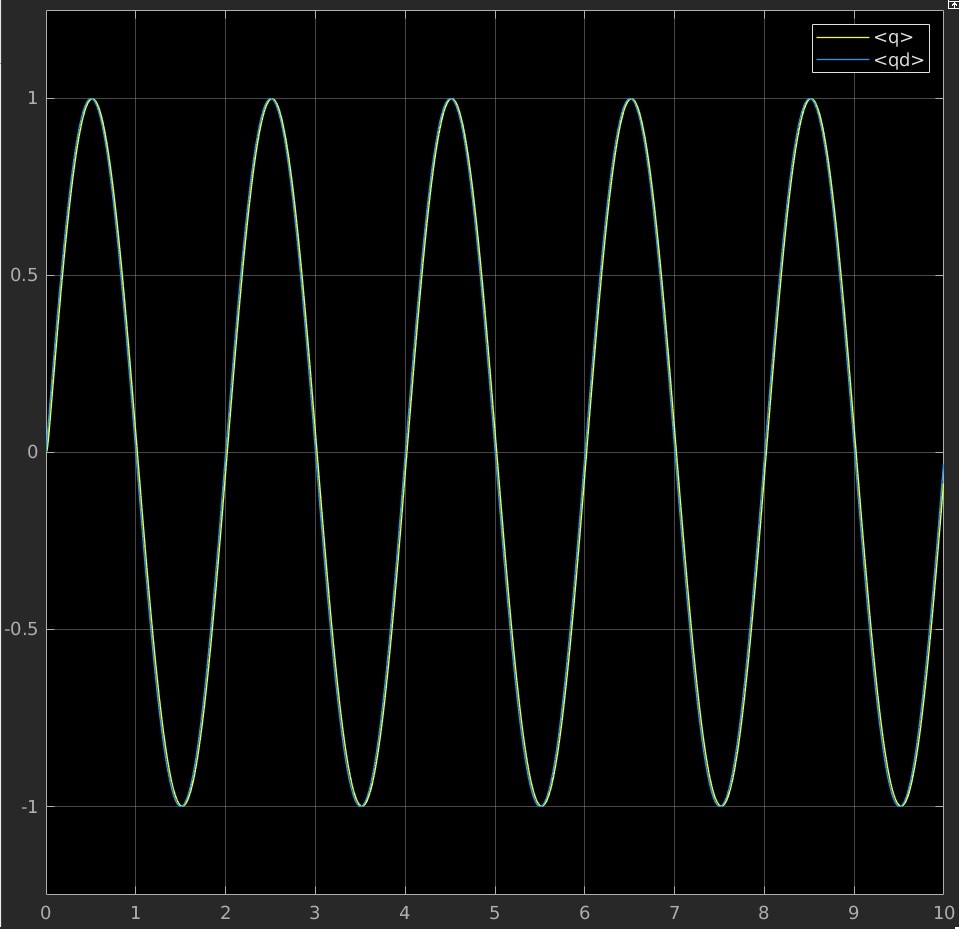
\includegraphics[keepaspectratio,width=0.6\textwidth]{adaptive_pos}
\caption{Adaptive control - position reference tracking}
\end{figure}

\begin{figure}[H]
\centering
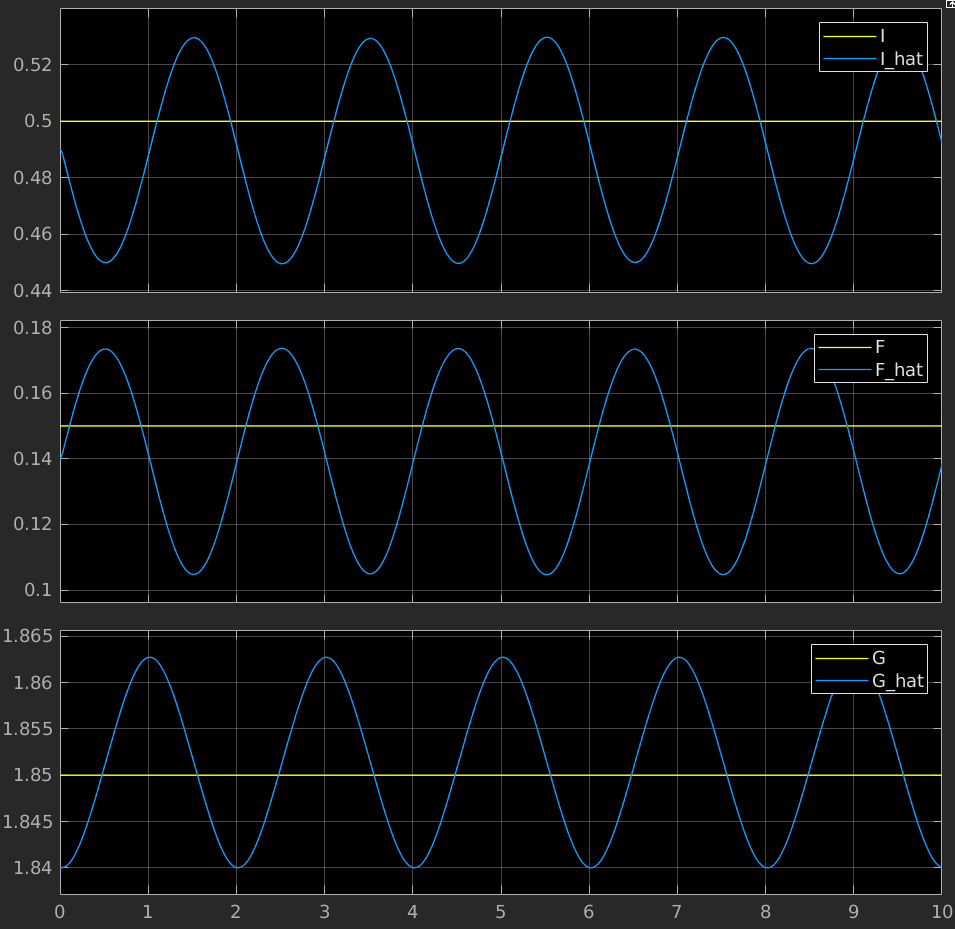
\includegraphics[keepaspectratio,width=0.6\textwidth]{adaptive_theta}
\caption{Adaptive control - parameter estimation}
\end{figure}
